\documentclass{report}

\usepackage[ngerman]{babel}
\usepackage[utf8]{inputenc}
\usepackage[T1]{fontenc}
\usepackage{hyperref}
\usepackage{csquotes}
\usepackage[a4paper]{geometry}
\usepackage{graphicx}

\usepackage[
    backend=biber,
    style=apa,
    sortlocale=de_DE,
    natbib=true,
    url=false,
    doi=false,
    sortcites=true,
    sorting=nyt,
    isbn=false,
    hyperref=true,
    backref=false,
    giveninits=false,
    eprint=false]{biblatex}
\addbibresource{../references/bibliography.bib}


\title{Ethik im Umgang mit Daten} 
\author{Ruben Nussbaumer}
\date{\today}


\begin{document}

\maketitle

\abstract{
    In diesem Dokument zeige ich auf, wie KI funktioniert und was KI überhaupt ist. 
    Danach erkläre ich und zeige ich auf, wie KI im Zusammenhang mit Ethik steht und habe noch einige Fragen zu diesem Thema beantwortet, wie z.B. bei welchen Sachen KI ein Ethisches Gewissen braucht usw.
}

\tableofcontents

\chapter{Einleitung}
Haben Sie sich schon einmal gefragt, wie KI funktioniert und ob KI auch eine Art Persöhnlichkeit haben kann und somit auch Entscheidungen treffen, die normalerweise Gefühle brauchen.
Ob und wie KI mit Ethischen Entscheidungen funktioniert und welche positiven und negativen Auswirkungen das haben kann, beantworte ich in diesem Paper.
Da das selber meine erste Auseinandersetzung mit KI und Ethik ist, habe ich selbst sehr viel gelernt, bei dieser Arbeit.
Diese Arbeit dient dazu, dass man sich einen Überblick machen über dieses Thema machen kann und danach kann man sich selbst vertiefen, wenn man möchte.
\section{Was ist eine KI?}
Künstliche Intelligenz (KI) ist ein Teilgebiet der Informatik. Sie imitiert menschliche kognitive Fähigkeiten, indem sie Informationen aus Eingabedaten erkennt und sortiert. Diese Intelligenz kann auf programmierten Abläufen basieren oder durch maschinelles Lernen erzeugt werden

\section{Wie funktioniert KI?}
KI beinhaltet eine grosse Zahl an Technologien, die das Ziel hat Maschinen und Computern die Fähigkeit
zu geben, Aufgaben, welche Menschen Zeit braucht, selbstständig zu erledigen, was normalerweise eine Menschliche Intelligenz benötigt.
Die Grundlegenden Konzepte, wie KI mit diesen Technologien beschaffen ist, sind in den folgenden Abschnitten beschrieben.
\subsection{Daten}
Die Grundlagen, die KI braucht um überhaupt zu funktionieren, sind Daten. KI bezieht ihr Wissen und die Infos, die sie braucht aus Daten, 
die ihr eingeschleust wurden.
\subsection{Maschinelles Lernen}
KI lernt viel durch Maschinelles Lernen. Sie haben sicher schon einmal gesehen, wie eine KI in einem Spiel platziert wird und diese solange
das Spiel zu verstehen lernt, bis es das ganze Spiel spielen kann. z.B. bei Super Mario.

\subsection{Neuronale Netzwerke}
Neuronale Netzwereke sind eine der bekanntsten Art von KI. Neuronale Netzwerke basieren auf der Funktionsweise vom menschlichen Gehirn. Die Netzwerke bestehen aus ganz vielen verbundenen Konten (Neuronen), welche in sogenannten Schichten organisisiert werden. 
Es gibt die Eingabeschicht, verborgene Schichten und die Ausgabeschicht. Jedes Neuron erhält Signale und bearbeitet diese durch gewichtete Verbindungen und leitet ein Signal weiter. Diese Gewichte werden während des Trainings angepasst, damit das Netzwerk noch genauer funktioniert.
 Mit Aktivierungsformen kann man mit Neuronalen Netzwerken Bzeihungen in den Daten erstellen, also Zusammenhänge zwischen Daten erkennen lassen. Tiefe neuronale Netzwerke mit ganz vielen Schichten werden als deep learning bezeichnet und erkennen sehr Komplexe Zusammenhänge. 
 Das verwendet man z.B bei Bilderkennung. Wenn ein Netzwerk trainiert ist, kann man es benutzen um Vorhersagen usw. zu treffen mit neuen Daten.

\subsection{Deep Learning}
Deep learning ist eine fortgeschrittene Methode des Maschinellen Lernens, welche tiefe neuronale Netzwerke verwendet, um umfangreiche Muster in sehr grossen Datenmengen zu erkennen. Die neuronalen Netzwerke haben viele Schichten von Neuronen, welche Automatisch dazu lernen, was wichtig ist und man braucht keinen Menschen dazu. Deep Learning benutzt man mit Neuronalen Netzwerken um Bilderkennnung und Spracherkennung usw. zu betreiben.
\subsection{Anwendungen der KI}
\begin{itemize}
    \item KI kann dabei helfen, die Fehlereffekte zu reduzieren.
    \item Spracherkennung
    \item Bildverarbeitung
    \item Automatisierung
    \item Empfehlungen auf persöhnlichen Interessen basierend
    \item Spieleintelligenz
\end{itemize}
\begin{figure}[h]

    \centering 
 
    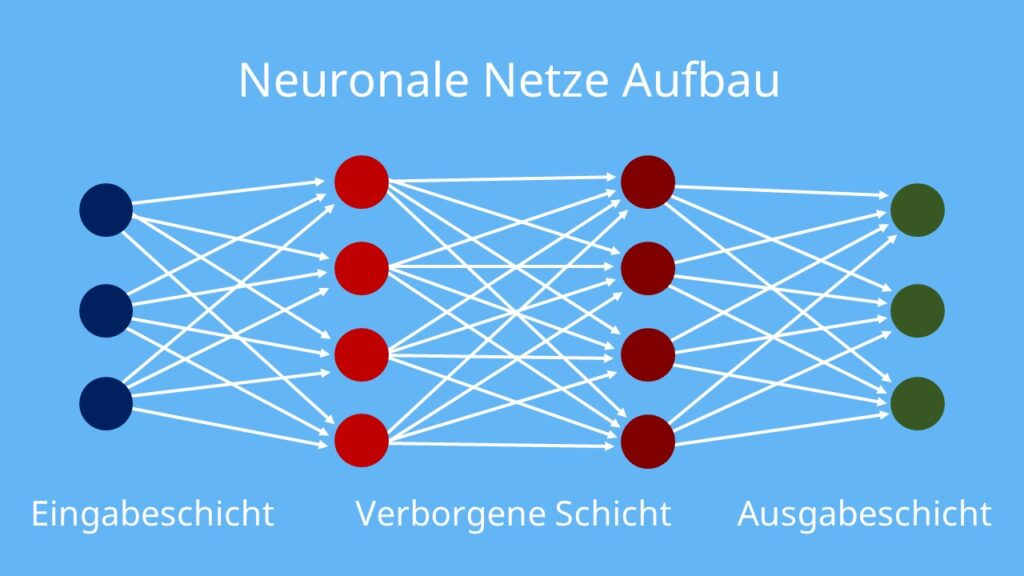
\includegraphics[width=0.65\textwidth]{img.jpg} 
 
    \caption{Neurale-Netzwerk-Grafik, IBM}
 
    \label{fig:meme}
 
 \end{figure}
 

\chapter{KI und Ethik}
Künstliche Intelligenz (KI) ist ein Teilgebiet der Informatik. Sie imitiert menschliche kognitive Fähigkeiten, indem sie Informationen aus Eingabedaten erkennt und sortiert. Diese Intelligenz kann auf programmierten Abläufen basieren oder durch maschinelles Lernen erzeugt werden

\printbibliography

\end{document}
